\documentclass[a4paper, 11pt]{article}
\input{macro/package.tex}
\input{macro/environement}
% Header et footer

\pagestyle{fancy}
\fancyhead{}
\fancyfoot{}
\renewcommand{\headwidth}{\textwidth}
\renewcommand{\footrulewidth}{0.4pt}
\renewcommand{\headrulewidth}{0pt}
\renewcommand{\footruleskip}{5px}

\fancyfoot[R]{Olivier Glorieux}
%\fancyfoot[R]{Jules Glorieux}

\fancyfoot[C]{ Page \thepage }
\fancyfoot[L]{1BIOA - Lycée Chaptal}
%\fancyfoot[L]{MP*-Lycée Chaptal}
%\fancyfoot[L]{Famille Lapin}

\input{macro/newcommand.tex}
\geometry{hmargin=2.0cm, vmargin=2cm}



\newcommand{\type}{TD }
\excludecomment{correction}
%\renewcommand{\type}{Correction TD }


\author{Olivier Glorieux}


\begin{document}

\title{\type 1 - Fonctions usuelles}

\section*{Entraînements}

\begin{exercice} 
\`{A} l'aide d'une \'etude de fonction, d\'emontrer les in\'egalit\'es suivantes:
\begin{enumerate}
\item $\forall \ddp x>0,\ x-\frac{x^2}{2}\leq \ln{(1+x)}\leq x$
\item $\forall \ddp x\in\R^+$: $e^x-\ddp\frac{x^2}{2}\geq 1$.
\end{enumerate}
\end{exercice}


\begin{correction}  \; \textbf{Utilisation d'une \'etude de fonction.}\\
\begin{enumerate}
\item \textbf{Montrons que $\mathbf{\forall x>0,\ddp\ x-\frac{x^2}{2}\leq \ln{(1+x)}\leq x}$:}\\
\noindent On d\'emontre l'in\'egalit\'e en deux temps.
\begin{itemize}
\item[$\bullet$] Montrons d'abord que pour tout $x>0$: $x-\ddp\frac{x^2}{2}\leq \ln{(1+x)}$:\\
\noindent On pose pour cela la fonction $f(x)=\ln{(1+x)}-x+\ddp\frac{x^2}{2}$. Cette fonction est bien d\'efinie sur $\R^{+}$ et elle est d\'erivable sur $\R^{+}$ comme compos\'ee et somme de fonctions d\'erivables. On obtient pour tout $x\geq  0$: $f^{\prime}(x)=\ddp\frac{1}{1+x}-1+x=\ddp\frac{x^2}{1+x}$. Comme on est sur $\R^{+}$, on a: $f^{\prime}(x)\geq 0$. On obtient donc les variations suivantes en utilisant le fait que $f(0)=0$: 
\begin{center}
\begin{tikzpicture}
 \tkzTabInit[espcl=5]{ $x$          /1,
       $f^{\prime}(x)$    /1,
       $f(x)$            /2}
     { $0$ ,$+\infty$}
  \tkzTabLine {,$+$,}
  \tkzTabVar{
       -/ $0$        /,
       +/           /
                      }
\end{tikzpicture}
\end{center}
Ainsi $0$ est le minimum de $f$ sur $\R^{+}$ et on obtient bien que pour tout $x>0$: $\ln{(1+x)}-x+\ddp\frac{x^2}{2}\geq 0$, \`{a} savoir $x-\ddp\frac{x^2}{2} \leq \ln{(1+x)}$.
\item[$\bullet$] On montre de m\^eme la deuxi\`eme in\'egalit\'e en \'etudiant la fonction $g(x)=\ln{(1+x)}-x$.
\end{itemize}
%---
\item \textbf{Montrons que $\mathbf{\forall x\in\R^+,\ e^x - \ddp \frac{x^2}{2}\geq 1}$:}\\
\noindent Pour tout $x\in\R^+$, on pose $f(x)=e^x-\ddp \frac{x^2}{2}-1$. La fonction $f$ est d\'efinie et d\'erivable sur $\R$ comme somme de fonctions d\'efinies et d\'erivables. On a, pour tout $x\in\R$,
$$f^{\prime}(x)=e^x-x.$$
Or on a montr\'e dans le cours (il faudrait refaire le raisonnement) que l'on a $e^x \geq x+1$ pour tout $x \in \R$, donc on a $f'(x) \geq 0$ sur $\R^+$. On obtient alors le tableau de variation suivant
\begin{center}
\begin{tikzpicture}
 \tkzTabInit{ $x$          /1,
       $f^{\prime}(x)$    /1,
       $f(x)$            /2}
     { $0$ ,$+\infty$}
  \tkzTabLine {,$+$,}
  \tkzTabVar{
        -/$0$           /,
       +/ $+\infty$          /
                      }
\end{tikzpicture}
\end{center}
Justifions les limites aux bornes: on a: $f(0)=e^0-0-1=0$. L'\'etude en $+\infty$ fait appara\^{i}tre une forme ind\'etermin\'ee. Pour lever l'ind\'etermination, on met en facteur le terme dominant \`{a} savoir $e^x$ et on obtient ainsi: $f(x)=e^x\left( 1-\ddp\frac{x^2}{2e^x}-\ddp\frac{1}{e^x}  \right)$. Par croissance compar\'ee, on sait que $\lim\limits_{x\to +\infty} \ddp\frac{x^2}{2e^x}=0$. Ainsi par quotient, somme et produit de limite, on obtient que $\lim\limits_{x\to +\infty}  f(x)=+\infty$.\\
\noindent Ainsi, $0$ est le minimum de $f$ atteint en $x=0$ et donc la fonction $f$ est toujours positive ou nulle. Ainsi, on a bien 
$$\fbox{$ \forall x\in \R,\ e^x\geq \ddp \frac{x^2}{2}+1. $}$$
%\item \textbf{Montrons que $\mathbf{\forall x\in\R,\ e^x\geq x+1}$:}\\
%\noindent \'Etude de l'in\'equation avec l'exponentielle.
%Pour tout $x\in\R$, on pose $f(x)=e^x-x-1$. La fonction $f$ est d\'efinie et d\'erivable sur $\R$ comme somme alg\'ebrique de fonctions d\'efinies et d\'erivables. On a, pour tout $x\in\R$,
%$$f^{\prime}(x)=e^x-1.$$
%\'Etudions donc le signe de $e^x-1$:
%$$e^x-1>0\Leftrightarrow e^x>e^0\Leftrightarrow x>0$$
%car la fonction $\ln{}$ est strictement croissante sur $\R^{+\star}$.
%On obtient alors le tableau de variation suivant
%\begin{center}
%\begin{tikzpicture}
% \tkzTabInit{ $x$          /,%
%      % $\sin{x}$     /,%
%      % $\sin{(2x)}$       /,
%       $f^{\prime}(x)$    /,
%       $f(x)$            /2}%
%     { $-\infty$ , $0$ ,$+\infty$}%
%  \tkzTabLine {,$-$,0,$+$,}%
%  %\tkzTabLine{ 0,$+$,0,$-$,0}
%  % \tkzTabLine{ 0,$+$,0,$-$,0}
%  \variation{
%     % {-/ $1$       /,%
%       +/ $+\infty$        /,
%        -/$0$           /,%
%       +/ $+\infty$          /
%                      }
%\end{tikzpicture}
%\end{center}
%Justifions les limites aux bornes: on a: $f(0)=e^0-1=0$. De plus $\lim\limits_{x\to -\infty} f(x)=+\infty$ comme sommes de limites. L'\'etude en $+\infty$ fait appara\^{i}tre une forme ind\'etermin\'ee. Pour lever l'ind\'etermination, on met en facteur le terme dominant \`{a} savoir $e^x$ et on obtient ainsi: $f(x)=e^x\left( 1-\ddp\frac{x}{e^x}-\ddp\frac{1}{e^x}  \right)$. Par croissance compar\'ee, on sait que $\lim\limits_{x\to +\infty} \ddp\frac{x}{e^x}=0$. Ainsi par quotient, somme et produit de limite, on obtient que $\lim\limits_{x\to +\infty}  f(x)=+\infty$.\\
%\noindent Ainsi, $0$ est le minimum de $f$ atteint en $x=0$ et donc la fonction $f$ est toujours positive ou nulle. Ainsi, on a bien 
%$$\fbox{$ \forall x\in \R,\ e^x\geq x+1. $}$$
%\item \textbf{Montrons que $\mathbf{\forall x\in\R^+,\ \sin{x}\leq x}$:}\\
%\noindent Pour cela on pose pour tout $x\in\R^+$: $f(x)=\sin{(x)}-x$. On va alors \'etudier les variations de cette fonction afin de montrer qu'elle est toujours n\'egative sur $\R^+$.
%\begin{itemize}
%\item[$\bullet$] La fonction $f$ est bien d\'efinie sur $\R$ donc en particulier sur $\R^+$.
%\item[$\bullet$] La fonction $f$ est d\'erivable sur $\R^+$ comme somme de fonctions d\'erivables. Et pour tout $x\in\R^+$, on a: $f^{\prime}(x)=\cos{(x)}-1$. Comme pour tout $x\in\R$, on a: $-1\leq \cos{(x)}\leq 1$, on obtient en particulier que pour tout $x\in\R^+$: $\cos{(x)}-1\leq 0$. Ainsi pour tout $x\in\R^+$: $f^{\prime}(x)\leq 0$.
%\item[$\bullet$] Tableau de variation:
%\begin{center}
%\begin{tikzpicture}
% \tkzTabInit[espcl=5]{ $x$          /,%
%      % $\sin{x}$     /,%
%      % $\sin{(2x)}$       /,
%       $f^{\prime}(x)$    /,
%       $f(x)$            /2}%
%     {$0$ ,$+\infty$}%
%  \tkzTabLine {,$-$,}%
%  %\tkzTabLine{ 0,$+$,0,$-$,0}
%  % \tkzTabLine{ 0,$+$,0,$-$,0}
%  \variation{
%     % {-/ $1$       /,%
%       +/ $0$        /,
%        -/           /%
%      % +/ $+\infty$          /
%                      }
%\end{tikzpicture}
%\end{center}
%\item[$\bullet$] Ainsi 0 est le maximum de $f$ sur $\R^+$ atteint en $x=0$. Donc pour tout $x\in\R^+$: $f(x)\leq 0$ ce qui est bien \'equivalent \`{a}: \fbox{$ \forall x\in\R^+,\ \sin{(x)}\leq x .$}
%\end{itemize}
\end{enumerate}
\end{correction}








\begin{exercice}  \;
Pour chacune des expressions, donner le domaine de d\'efinition et simplifier quand c'est possible.
\begin{enumerate}
\item $f(x)=x\ln{\ddp\sqrt{e^{\frac{x}{2}}}}+\left( \ddp\sqrt{e^{2\ln{(2x-1)}}} \right)^3.$ 
\item $g(x)=e^{\ddp\sqrt{\ln{x}}}+e^{(\ln{x})^2}.$
\end{enumerate}
\end{exercice}





\begin{correction}  \;
\begin{enumerate}
 \item
$f(x)=x\ln{\ddp\sqrt{e^{\frac{x}{2}}}}+\left( \ddp\sqrt{e^{2\ln{(2x-1)}}} \right)^3$: La fonction $f$ est bien d\'efinie si et seulement si $\sqrt{e^{\frac{x}{2}}}>0$, $e^{\frac{x}{2}}\geq 0$, $2x-1>0$ et $e^{2\ln{(2x-1)}}\geq 0$. Comme toute exponentielle est strictement positive, la fonction $f$ est bien d\'efinie si et seulement si $2x-1>0\Leftrightarrow x>\ddp\demi$. Ainsi \fbox{$\mathcal{D}_f=\rbrack \ddp\demi,+\infty\lbrack$}.\\
\noindent  Pour tout $x>\ddp\demi$, on a: 
$$f(x)=x\ln{  \left( e^{\frac{x}{2}} \right)^{\demi} } + \left( e^{2\ln{(2x-1)}}\right)^{\frac{3}{2}}= x\ln{( e^{\frac{x}{4}} )}  +  \left( e^{\ln{((2x-1)^2)}}\right)^{\frac{3}{2}}= x\times \ddp\frac{x}{4}+ ((2x-1)^2)^{\frac{3}{2}}= \ddp\frac{x^2}{4}+(2x-1)^3$$
\item 
$g(x)=e^{\ddp\sqrt{\ln{x}}}+e^{(\ln{x})^2}$. La fonction $g$ est bien d\'efinie si et seulement si $x>0$ et $\ln{x}\geq 0\Leftrightarrow x\geq 1$. Ainsi \fbox{$\mathcal{D}_g=\lbrack 1,+\infty\lbrack$}.\\
\noindent On ne peux RIEN simplifier car $\sqrt{\ln{x}}=\left( \ln{x} \right)^{\demi}\not= \ddp\demi\ln{(x)}$... De m\^{e}me, on a: $(\ln{x})^2\not= \ln{(x^2)}$... et on ne peux rien faire avec $(\ln{x})^2$.
\end{enumerate}
\end{correction}



\begin{exercice}
    Etudier les fonctions suivantes : 

    \begin{enumerate}
        \item $f_1 :\ddp x\mapsto (2x^2-4x+5)e^x-xe^{(x^2)} $
        \item $f_2 :\ddp x\mapsto \ln(x^2+x+1)-x$
        \item $f_3 :\ddp x\mapsto xe^{-x^2+x}$
        \item $f_4 :\ddp x\mapsto x^2e^{(-x^2)}$
        \item $f_5 :\ddp x\mapsto x\ln(x)$
        \item $f_6 :\ddp x\mapsto \frac{e^{x}}{e^{2x}+1}$
    \end{enumerate}
\end{exercice}


\section*{Type DS}


\begin{exercice}


\begin{enumerate}
\item Montrer à l'aide d'une étude de fonction  que pour tout $x\in \R$, $e^{x}\geq x+1$.
    \item En déduire que pour tout $x\in \R$, $e^{2x}-x\geq 0$
    \item De même en déduire que pour tout $x\in \R$, $e^{x}-2x\geq 0$
    \item Etudier la fonction $$f : x\mapsto \sqrt{e^{x}-2x}$$
    \item Etudier la fonction $$g : x\mapsto \sqrt{e^{2x}-x}$$
\end{enumerate}

\end{exercice}


\begin{correction}
    
\end{correction}


\begin{exercice}
Soit $f$ la fonction définie par 
$$f(x)= \frac{e^{x}}{\ln(x)} $$
\begin{enumerate}
\item Donner l'ensemble de définition et de dérivation de $f$. 
\item Calculer la dérivée de $f$ en déduire que le signe de $f'$ dépend de celui de $g(x)=\ln(x) - \frac{1}{x}$
\item Donner l'ensemble de définition et de dérivation de $g$ et calculer sa dérivée. 
\item Montrer qu'il existe un unique $\alpha\in ]1,+\infty[$ tel que $f'(x)>0$ sur $]\alpha, +\infty[$ et $f'(x)<0$ sur $]0,\alpha[\cap D_f$. 
\item Donner le tableau de variations complet de $f$. 
\item Donner l'équation de la tangente à la courbe représentative de $f$ en $e$.

\end{enumerate}
\end{exercice}

\begin{correction}
\begin{enumerate}
\item La fonction $\exp$ est définie  et dérivable sur $\R$. La fonction $ \ln$ est définie et dérivable sur $]0,+\infty[$. La fonction inverse est définie et dérivabel sur $\R^*$ et enfin $\ln(x) =0$ si et seulement si $x=1$ donc la fonction $f$ est définie  et dérivable sur $D_f= ]0,1[\cup]1,+\infty[$. 
\item On  a pour tout $x\in D_f$ 
$$f'(x)=\frac{e^x \ln(x)- e^x\frac{1}{x}}{\ln^2(x)} = \frac{e^x}{\log^2(x)} g(x) $$
Comme poru tout $x\in D_f$, $\frac{e^x}{\log^2(x)}\geq 0$, 
 le signe de $f'$ est égal à celui de $g(x)=\ln(x)-\frac{1}{x}$. 
 
 \item $g$ est définie et dérivable sur $]0,+\infty[$ et on a $g'(x)=\frac{1}{x}+\frac{1}{x^2}$ Ainsi $g'(x)$ est positif prou tout $x\in  ]0,+\infty[$. 
 
 \item La fonciton $g$ est strictement croissante. Comme $\lim_{x\tv 
 0} g(x)  = -\infty$ $\lim_{x\tv 
 \infty } g(x)  = \infty$, le théorème de la bijection assure qu'il existe un unique $\alpha \in ]0,+\infty[ $ tel que $g(\alpha) =0$ 
 
 Comme $g(1) = -1 < 0$ et que $g$ est strictement croissante, on a de plus $\alpha>1$ 

 \item 
\begin{center}
\begin{tikzpicture}
\tkzTabInit[espcl=6]{$x$ / 1,Signe de\\$f'(x)$/1, Variations de\\ $f$ / 3}%
{$0$, $1$, $+\infty$}%
\tkzTabLine{,-,h,+, }
\tkzTabVar{+/$0$ , -/$-\infty$,+/$+\infty$ }
   \end{tikzpicture}
\end{center}


\item On a $f'(e) = e^e g(e) = -e^e(1-\frac{1}{e})  =-e^{e}+e^{e-1}$ et $f(e) = e^{e}$
Donc l'équation de la tangente à la courbe représentative de $f$ en $e$ et donnée par 
$$y-e^{e} =(-e^{e}+e^{e-1} )(x-e)$$
\end{enumerate}
\end{correction}


%------------------------------------------------------------------------------------
%------------------------------------------------------------------------------------
%------------------------------------------------------------------------------------
%------------------------------------------------------------------------------------
%------------------------------------------------------------------------------------



\begin{exercice}[BAC 1997 PONDICHERY]
   

\medskip

On considère la fonction $f$ définie sur $[0~;~+\infty[$ par

\[f(x)=\dfrac{\text{e}^{x}-1}{x\text{e}^{x}+1}\]

On désigne par $\mathcal{C}$ sa courbe représentative dans le plan rapporté
à un repère orthonormal (O,$\vec{i}$,$\vec{j}$)

\bigskip

\textbf{Partie A}

\medskip

\textbf{$\star$} \textbf{étude d'une fonction auxiliaire}

\medskip

Soit la fonction $g$ définie sur l'intervalle $[0~;~+\infty[$ par

\[g(x) = x + 2 - \text{e}^{x}.\]

\begin{enumerate}
\item Étudier le sens de variation de $g$ sur $[0~;~+\infty[$ et déterminer la limite de $g$ en $+\infty$.
\item
\begin{enumerate}
\item Montrer que l'équation $g(x)=0$ admet une solution et
une seule dans $[0~;~+\infty[$.

On note $\alpha$ cette solution.
\item Prouver que $1< \alpha<2$. (On rappelle que $2<e<3$)
\end{enumerate}
\item En déduire le signe de $g(x)$ suivant les valeurs de
$x$.
\end{enumerate}

\bigskip

\textbf{Partie B} 

\medskip

\textbf{$\star$} \textbf{Étude de la fonction $f$ et tracé de la courbe $\mathcal{C}$}

\medskip

\begin{enumerate}
\item 
	\begin{enumerate}
		\item Montrer que, pour tout $x$ appartenant à
$[0~;~+\infty[$,

\[f\,^{\prime}(x)=\frac{\text{e}^{x}g(x)}{(x\text{e}^{x}+1)^{2}}.\]
\item En déduire le sens de variation de la fonction $f$ sur
$[0~;~+\infty[$.
\end{enumerate}
\item
	\begin{enumerate}
		\item Montrer que pour tout réel positif $x$,
\[
f(x)=\frac{1- \text{e}^{-x}}{x+\text{e}^{-x}}%
\]
		\item En déduire la limite de $f$ en $+\infty$.
Interpréter graphiquement le résultat trouvé.
	\end{enumerate}
\item
	\begin{enumerate}
		\item Établir que $f(\alpha) = \displaystyle\frac{1}{\alpha+
1}$.
		\item En utilisant l'encadrement de $\alpha$ établi dans la
question \textbf{A.2.}, donner un encadrement de $f(\alpha)$.
	\end{enumerate}
\item Déterminer une équation de la tangente (T) à la
courbe $\mathcal{C}$ au point d'abscisse 0.
\item
	\begin{enumerate}
		\item Établir que, pour tout $x$ appartenant à
l'intervalle $[0~;~+\infty[$,

\[f(x)-x=\frac{(x+1)\,u(x)}{x\text{e}^{x}+1}\quad \text{avec}\: u(x) = \text{e}^{x} - x\text{e}^{x}-1.
\]
		\item Étudier le sens de variation de la fonction $u$ sur
l'intervalle $[0~;~+\infty[$. En déduire le signe de $u(x)$.
		\item Déduire des questions précédentes la position
de la courbe $\mathcal{C}$ par rapport à la droite (T).
	\end{enumerate}
\item Tracer $\mathcal{C}$ et (T).
\end{enumerate}



\end{exercice}





\end{document}